\chapter{Vaatimustenkeruusuunnitelma} % Itse luvun otsikko. Huom ei numeroa!
\label{keruu} % Tähän kappaleeseen voi viitata \ref{keruu}
\thispagestyle{fancy} % Tarvitaan, jotta header/footer näkyvät otsikkosivuilla

Tässä luvussa käsitellään jo olemassa olevia dokumentaatioita, ja mitä vaatimuksia asiakastietojärjestelmälle voidaan niiden perusteella määrittää. Luvussa esitellään erilaisia tapoja, joita voidaan hyödyntää vaatimusten keruussa sidosryhmiltä.

\section{Taustatilanne}

% TODO pitäisiköhän tähän vielä lisätä jotain?
Megantti konsernilla ei ennestään ollut käytössä keskitettyä asiakkuudenhallintajärjestelmää (\acrshort{crm}).
Asiakastietoja ovat keränneet lähinnä myyntipuolen työntekijät, joilla on ollut ongelmia tietojen jakamisessa keskenään sekä asiakastietojen tietosuojaan liittyen. Uuden CRM:n olisi tarkoitus keskittää tietojen hallinnointi ja tasapuolistaa erityisesti eri myyntihenkilöiden informatiivista asemaa asiakkaita kohtaan.

\section{Nykyisen dokumentaation analyysi}
Tässä kappaleessa analysoidaan olevassa olevaa dokumentaatiota. Tämän analyysin pohjalta määritetään alustavia vaatimuksia.


    \subsection{Kehyskertomuksen analyysi}
    Con-Salting Oy on kerännyt alustavia vaatimuksia kehyskertomukseen. Kehyskertomuksessa määritetään asiakastietojärjestelmälle alustavia vaatimuksia. Kehyskertomuksen perusteella voidaan määrittää sidosryhmiä, jotka tulee ottaa huomioon, ja joiden kanssa tulee kommunikoida vaatimuksia määriteltäessä.

    Tällaisia sidosryhmiä ovat muun muassa yrityksen johto ja myynti- ja markkinointiosasto.
    sidosryhmät ovat esittäneet toivomuksina esimerkiksi asiakastietojärjestelmän nopean toiminnan, käytettävyyden erilaisilta päätelaitteilta sekä asiakkaan 
    automaattisen profiloinnin. 
        
    Kehyskertomuksessa ilmenee myös muita asioita jotka tulee ottaa huomioon:
    
    \begin{itemize}
        \item Järjestelmän tulee olla yhteensopiva muiden yrityksen järjestelmien kanssa kuten yrityksen varastojärjestelmän kanssa.
	\item Asiakastietojärjestelmän tulee myös olla \gls{gdpr} mukainen
        \item Järjestelmän tulee pystyä hoitamaan joitain asioita automaattisesti, kuten suurostobonukset.
    \end{itemize}

    Nämä vaatimukset ovat kuitenkin ainoastaan suuntaan antavia, ja niitä tulee tarkentaa vaatimustenkeruussa. 


\section{Vaatimustenkeruumetodit}

    Vaatimustenkartutusmetodit voidaan jakaa kahteen eri osa-alueeseen: Epäsuoriin- ja suoriin metodeihin.
    Tässä kappaleessa käsitellään Megantin asiakastietojärjestelmän kehitystä varten käytettäviä metodeja.


    \section*{Suorat metodit}

        Suorissa kartutustekniikoissa järjestelmän vaatimuksia kartoitetaan yhdessä sidosryhmien kansssa.
        Seuraavia suorakartutustekniikoita hyödynnetään mahdollisimman kattavan analyysin toteuttamiseen:

        \subsubsection*{Haastattelut}

            Sidosryhmille järjestetään kahdentyyppisiä haastatteluja. Ensimmäisessä haastattelussa haastateltavat vastaavaat ennaltamääriteltyihin kysymyksiin. 
            Ensimmäisten kysymysten on takroitus on luoda selkeä kuva nykytilanteesta ja sen mahdollisista ongelmakohdista. Toisessa haastattelussa haastattelu toteutetaan avoimesti. Haastateltaville esitetään erilaisia kysymyksiä järjestelmän toiminnalisuuteen liittyen jolloin haastateltavien kanssa voidaan vuorovaikutteisesti pohtia millainen järjestelmän tulisi olla.

        \subsubsection*{Havainnointi}

            Meganttiin lähetetään 2 kehitystiimiläistä tarkkailemaan. Nämä tiimiläiset seuraavat noin kahden viikon ajan Megantin työntekijöiden työtä, ja tekevät 
            muistiinpanoja työntekijöiden tarpeista järjestelmään liittyen. He havainnoivat myös mitä puutteita ja vahvuuksia nykyisessä asiakastietojärjestelmässä on ja raportoivat näistä suoraan prototyyååien kehitystiimille. Havainnointi tiedonkeruumenetelmänä on tärkeää, sillä ihmisten on usein vaikea pukea arkipäivän työntekoa sanoiksi. Havainnoinnin avulla pystymme rakentamaan järjestelmän, joka vastaa myös tosielämän tarpeita.


        \subsubsection*{Ryhmätapaamiset}

            Projektin aikana järjestetään tapaamisia sidosryhmien kanssa. Näissä tapaamisissa kehitystiimi on suoraan kontaktissa kyseisen ryhmän kanssa ja ryhmän on mahdollista kertoa asiakastietojärjestelmän nykytilasta, kuvailla tilanteita ja havainnollistaa kuinka he haluaisivat järjestelmän toimivan kyseisissä tilanteissa.


    \section*{Epäsuorat metodit}

        Epäsuorissa kartutustekniikoissa sidosryhmiin ei olla suorassa kontaktissa, vaan käytetään jo ennalta olevia tietoja.
        Käytämme seuraavia epäsuoriakartutustekniikoita:

        \subsubsection*{Taustatutkimus}

        Con-Salting Oy on kerännyt jo muutamia yrityksen vaatimuksia kehyskertomukseen. 
        Näitä vaatimuksia ovat esimerkiksi asiakastietojen ylläpito, ja asiakkaiden profilointi.
        Vaatimukset ovat kuitenkin löysästi määriteltyjä ja vaativat tarkennusta.

	Kartoittaa tulee ainakin nykyiset käytössä olevat järjestelmät (tietokannat, ohjelmistot jne), jotta saadaan tietoon mitä vanhoja järjestelmiä voidaan suoraan korvata uudella ja mitkä vanhat järjestelmät ovat tuotannon kannalta välttämättömiä, ja joiden kanssa uuden järjestelmän tulisi olla yhteensopiva.

        \subsubsection{Kyselyt}

        Osalle järjestelmän sidosryhmistä järjestetään kyselyitä, jossa selvitetään heidän mielestään tärkeimpiä järjestelmän vaatimuksia.
        Tällaisia sidosryhmiä ovat sisäiset käyttäjät, kuten yrityksen johto-, asiakaspalvelu- ja järjestelmän ylläpitohenkilöstö.

        \subsubsection*{Prototyypit}

        Sisäisille käyttäjille valmistetaan kahteen otteeseen prototyyppi järjestelmästä. Ensimmäisen vaiheen prototyypin on tarkoitus varmistaa yhteensopivuus vanhojen järjestelmien kanssa ja varmistaa ettei olennaisia komponentteja puutu valmiista järjestelmästä. Toisen vaiheen prototyyppi keskittyy ominaisuuksien hiomiseen ja tässä vaiheessa kehitystä ohjaa vahvasti erinäiset ryhmätapaamiset ja haastattelut käyttäjien kanssa.
	
\section{Sidosryhmäanalyysi}

        Kuvassa \ref{img:sidosryhmat} (sivulla \pageref{img:sidosryhmat}) on esitelty erilaisia ohjelmistoon liittyviä sidosryhmiä ajatuskartan muodossa.
	% TODO tähän kohtaan lisää tekstiä

        \begin{figure}[H] % tämä H tarkoittaa tekstin mukana { h | t | b | p | H}
		\centering
		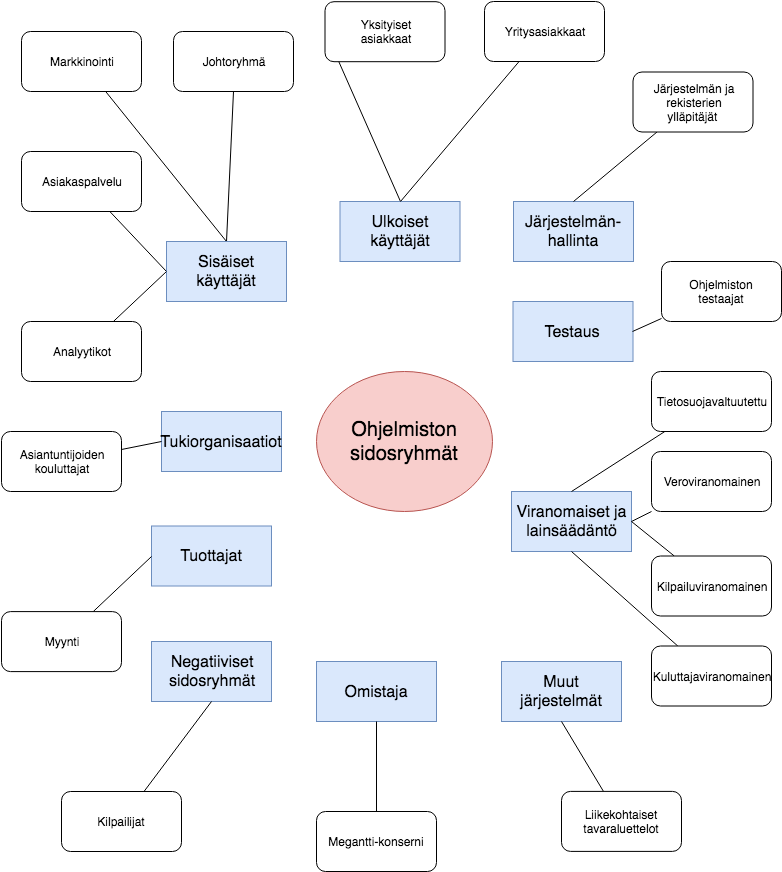
\includegraphics[width=\textwidth]{sidosryhmat.png}
		\caption{Ohjelmiston sidosryhmät} % Raportissa tulee olla selite jokaisen kuvan/kuvion/taulukon alla
		\label{img:sidosryhmat}
	\end{figure}
\section{Alustavat havaitut vaatimukset ja luokittelu}
Seuraavassa taulukossa on havainnollistettu alustavia vaatimuksia. Taulukossa on myös määritelty vaatimusten keskinäisiä tärkeysjärjestyksiä.

% Please add the following required packages to your document preamble:
% \usepackage[table,xcdraw]{xcolor}
% If you use beamer only pass "xcolor=table" option, i.e. \documentclass[xcolor=table]{beamer}
\begin{table}[]
    \begin{tabular}{llll}
    \multicolumn{4}{l}{Prioriteeti(1=Vähiten tärkeä, 2= Jonkin verran tärkeä, 3= Erittäin tärkeä)  Luokat(T=Tuottajat, H=Hyödyntäjät)}                                                                                                                                                                           \\ \hline
    \multicolumn{1}{|l|}{{\color[HTML]{000000} \textbf{Prioriteetti}}} & \multicolumn{1}{l|}{{\color[HTML]{000000} \textbf{Lähde}}} & \multicolumn{1}{l|}{{\color[HTML]{000000} \textbf{Luokka}}} & \multicolumn{1}{l|}{{\color[HTML]{000000} \textbf{Vaatimus}}}                                                \\ \hline
    \multicolumn{1}{|l|}{3}                                            & \multicolumn{1}{l|}{Haastattelut}                                      & \multicolumn{1}{l|}{T/H}                                    & \multicolumn{1}{l|}{Asiakastietojärjestelmää tulee pystyä käyttää eri päätelaitteilta.}                       \\ \hline
    \multicolumn{1}{|l|}{3}                                            & \multicolumn{1}{l|}{Taustatutkimus}                                      & \multicolumn{1}{l|}{T/H}                                    & \multicolumn{1}{l|}{Järjestelmän tulee noudattaa GDPR:ää.}                                                   \\ \hline
    \multicolumn{1}{|l|}{3}                                            & \multicolumn{1}{l|}{Taustatutkimus}                                      & \multicolumn{1}{l|}{T}                                      & \multicolumn{1}{l|}{Järjestelmän tulee olla yhteensopiva muiden olemassa olevien järjestelmien kanssa.}      \\ \hline
    \multicolumn{1}{|l|}{2}                                            & \multicolumn{1}{l|}{Havainnointi}                                      & \multicolumn{1}{l|}{T}                                      & \multicolumn{1}{l|}{Asiakkaiden tiedot tulee pystyä etsiä järjestelmästä nopeasti.}                           \\ \hline
    \multicolumn{1}{|l|}{3}                                            & \multicolumn{1}{l|}{Haastattelut}                                      & \multicolumn{1}{l|}{T}                                      & \multicolumn{1}{l|}{Järjestelmä rakennetaan olemassa olevan olevan ERP SQL constructoreiden päälle.}          \\ \hline
    \multicolumn{1}{|l|}{2}                                            & \multicolumn{1}{l|}{Prototyypit}                                      & \multicolumn{1}{l|}{T}                                      & \multicolumn{1}{l|}{Järjestelmän tulee seurata asiakkaiden ostoskäyttäytymistä.}                              \\ \hline
    \multicolumn{1}{|l|}{3}                                            & \multicolumn{1}{l|}{Havainnointi}                                      & \multicolumn{1}{l|}{T}                                      & \multicolumn{1}{l|}{Järjestelmän tulee pitää lokia kaikista tapahtumista.}                                   \\ \hline
    \multicolumn{1}{|l|}{2}                                            & \multicolumn{1}{l|}{Taustatutkimus}                                      & \multicolumn{1}{l|}{T}                                      & \multicolumn{1}{l|}{Järjestelmän pitää pystyä analysoida ja profiloida asiakkaita.}                         \\ \hline
    \multicolumn{1}{|l|}{1}                                            & \multicolumn{1}{l|}{Prototyypit/Haastattelut}                                      & \multicolumn{1}{l|}{T/H}                                    & \multicolumn{1}{l|}{Järjestelmän tulee olla helppokäyttöinen(Graphical user Interface.)}                    \\ \hline
    \multicolumn{1}{|l|}{1}                                            & \multicolumn{1}{l|}{Prototyypit}                                      & \multicolumn{1}{l|}{T/H}                                    & \multicolumn{1}{l|}{Järjestelmässä tulee olla monipuolisia toimintoja, kuten ostoshistoria, selainhistoria.}\\ \hline
    \multicolumn{1}{|l|}{2}                                            & \multicolumn{1}{l|}{Haastattelut}                                      & \multicolumn{1}{l|}{T/H}                                    & \multicolumn{1}{l|}{Järjestelmän luotettavuus tulee taata.}                                                 \\ \hline
    \multicolumn{1}{|l|}{1}                                            & \multicolumn{1}{l|}{Ryhmätapaamiset}                                      & \multicolumn{1}{l|}{H}                                    & \multicolumn{1}{l|}{Järjestelmän tulee pystyä yksilöllistää asiakkaan markkinointia.}                       \\ \hline
    \multicolumn{1}{|l|}{2}                                            & \multicolumn{1}{l|}{Ryhmätapaamiset}                                      & \multicolumn{1}{l|}{T}                                    & \multicolumn{1}{l|}{Järjestelmän tulee pitää kirjaa järjestelmätapahtumista.}                               \\ \hline
   

    \end{tabular}
    \end{table}	
    
\section{Vaatimusten keruuprojektin aikataulu (Gantt)}

	Vaatimusten keruun aikatulua on havainnollistettu Gantt-taulukon muodossa (Liitteessä \ref{aikatauluesimerkki}). Taulukosta ilmenee mikä vaatimusten keruumenetelmä on käytössä milloinkin.

